\documentclass[12pt]{article}
\usepackage[margin=1in]{geometry}
\usepackage{graphicx}
\usepackage{booktabs}
\usepackage{amsmath}
\usepackage{hyperref}
\usepackage{float}

\title{Replicating the LASSO Column of Table 4 from Varian (2014)}
\author{Tate Johnson \\ GSE 552 --- Causal Machine Learning}
\date{\today}

\begin{document}

\maketitle

% =============================================================================
\section{The Original Paper}
% =============================================================================

Varian (2014)\footnote{\url{https://doi.org/10.1257/jep.28.2.3}} is a widely
cited survey aimed at economists, arguing that machine learning techniques ---
including classification and regression trees, random forests, and penalized
regression methods such as LASSO, LARS, and elastic nets --- offer powerful
tools for prediction and variable selection that are underutilized in empirical
economics. The paper serves as an accessible introduction to a broad set of ML
methods, walking through each with applied examples and situating them relative
to familiar econometric tools.

The paper's central empirical demonstration focuses on cross-country economic
growth regressions. Using the dataset from Fernandez, Ley, and Steel (2001),
which contains 72 countries and 41 potential predictors of average GDP growth
over 1960--1985, Varian demonstrates that LASSO can identify important
predictors of economic growth as effectively as computationally exhaustive
methods --- including Bayesian model averaging across millions of model
specifications --- but at a fraction of the computational cost. The empirical
strategy is straightforward: fit a penalized regression (LASSO) with the
penalty parameter $\lambda$ selected by 10-fold cross-validation, and examine
which variables survive the shrinkage procedure and in what order they enter
the model.

% =============================================================================
\section{The Result of Interest}
% =============================================================================

I replicate the LASSO column of Table 4 in Varian (2014), which reports the
ordinal rank of importance among variables selected by LASSO for predicting
cross-country economic growth. The specific target result is:

\begin{itemize}
    \item Equipment investment: Rank 1
    \item Fraction Confucian: Rank 2
    \item Fraction Protestant: Rank 5
    \item Open economy: Rank 6
    \item Sub-Saharan dummy: Rank 7
    \item Fraction Muslim: Rank 8
    \item Degree of capitalism: Rank 9
    \item GDP level 1960, Life expectancy, Rule of law: zeroed out (dash)
\end{itemize}

This result is worth replicating for two reasons. First, it is the paper's
central quantitative claim --- that LASSO identifies the same important growth
predictors as Bayesian model averaging and Sala-i-Mart\'{i}n's (1997)
exhaustive CDF(0) approach, despite using a single penalized regression rather
than the two million regressions Sala-i-Mart\'{i}n (1997) required to reach
similar conclusions. The computational contrast is stark: LASSO achieves
comparable variable selection in a fraction of a second. Second, the LASSO
variable selection step is now understood to be the foundation of modern causal
ML pipelines. Belloni, Chernozhukov, and Hansen (2014) formalized the Double
LASSO estimator, which uses LASSO variable selection as the first stage of a
valid causal inference procedure in high-dimensional settings. Replicating
Varian's demonstration thus speaks directly to the role of LASSO as Step 1 in
causal ML.

% =============================================================================
\section{Data and Methods}
% =============================================================================

\subsection*{Data}

The data come from Fernandez, Ley, and Steel (2001), originally compiled by
Sala-i-Mart\'{i}n (1997) for a study of cross-country growth determinants.
The dataset contains 72 country observations and 42 variables: one outcome
variable ($y$, average GDP growth rate 1960--1985) and 41 covariates spanning
geographic, institutional, demographic, religious, and macroeconomic
characteristics. The raw data file (\texttt{FLS-data.csv}) is committed to
\texttt{input/} and is available from the Varian (2014) replication archive on
openICPSR (project 113925). The outcome variable has mean 2.07\% and standard
deviation 1.83\% across the 72 countries.

\subsection*{Preprocessing}

\texttt{code/preprocess.R} reads \texttt{input/FLS-data.csv}, performs
integrity checks (verifying 72 observations, 42 columns, and zero missing
values), separates the outcome variable $y$ from the 41 covariates $X$, and
writes the analysis-ready dataset to \texttt{temp/clean\_data.csv}. No
substantive transformations are applied --- the FLS dataset is already clean.

\subsection*{Analysis}

\texttt{code/analysis.R} reads \texttt{temp/clean\_data.csv} and implements
LASSO using the \texttt{glmnet} package (version 4.1-10) in R (version 4.5.1).
The analysis proceeds in two parts.

\textbf{Part I} replicates Varian's original result by hard-coding his
cross-validation-selected penalty parameter $\lambda = 0.1489$ and extracting
the non-zero LASSO coefficients ranked by magnitude. This exactly reproduces
the LASSO column of Table 4.

\textbf{Part II} runs 10-fold cross-validation using the current version of
\texttt{glmnet} to select $\lambda$ data-adaptively, yielding a different
optimal penalty ($\lambda = 0.0405$) and a less sparse model. The difference
between the two results illustrates the sensitivity of LASSO variable selection
to software versioning --- an important reproducibility finding in its own right.

The LASSO objective function minimized in both parts is:

\begin{equation}
\label{eq:lasso}
    \min_{\beta} \sum_{i=1}^{n} (y_i - x_i'\beta)^2 +
    \lambda \sum_{p=1}^{P} |\beta_p|
\end{equation}

where $y_i$ is the average GDP growth rate for country $i$, $x_i$ is the
vector of 41 standardized covariates, $\lambda$ is the penalty parameter, and
$|\beta_p|$ is the L1 penalty that shrinks irrelevant coefficients to exactly
zero. All outputs --- tables and figures --- are written programmatically to
\texttt{output/tables/} and \texttt{output/figures/} and pulled into this
document via \texttt{\textbackslash input\{\}} and
\texttt{\textbackslash includegraphics\{\}}.

% =============================================================================
\section{Replication Results}
% =============================================================================

\subsection*{Main Result: Replication of Table 4 LASSO Column}

Table~\ref{tab:main} replicates the LASSO column of Table 4 from Varian (2014)
--- which is itself based on Ley and Steel (2009), who applied Bayesian model
averaging to the same Sala-i-Mart\'{i}n (1997) growth dataset --- and compares
it against results from the updated \texttt{glmnet} version. At Varian's
original $\lambda = 0.1489$, we exactly reproduce his published rankings:
equipment investment enters first, fraction Confucian second, and GDP level
1960, life expectancy, and rule of law are all shrunk to exactly zero. The
replication is a complete success at the hard-coded $\lambda$.

\begin{table}[h]
\centering
\caption{Replication of Table 4 (LASSO Column): Variable Rankings for Predictors of Economic Growth}
\label{tab:main}
\begin{tabular}{lcc}
\hline
\textit{Predictor} & \textit{Varian (2014)} & \textit{Updated (glmnet 4.1-10)} \\
\hline
GDP level 1960 & - & 6 \\
Fraction Confucian & 2 & 2 \\
Life expectancy & - & 23 \\
Equipment investment & 1 & 1 \\
Sub-Saharan dummy & 7 & 8 \\
Fraction Muslim & 8 & 10 \\
Rule of law & - & 12 \\
Open economy & 6 & 11 \\
Degree of capitalism & 9 & 19 \\
Fraction Protestant & 5 & 7 \\
\hline
\multicolumn{3}{p{0.85\textwidth}}{\small \textit{Notes:} Rankings show the ordinal importance of each variable among those selected by LASSO. A dash indicates the variable was shrunk to exactly zero. Varian's results use $\lambda = 0.1489$ (original cross-validation, glmnet circa 2014). Updated results use $\lambda$ selected by cross-validation with glmnet 4.1-10.}
\end{tabular}
\end{table}


The updated \texttt{glmnet} (version 4.1-10) selects a smaller $\lambda =
0.0405$ via cross-validation, producing a less sparse model with 27 non-zero
coefficients compared to Varian's 14. Notably, variables that Varian zeroed
out --- GDP level 1960 (now rank 6), life expectancy (rank 23), and rule of law
(rank 12) --- are retained in the updated model, though at lower ranks. The
top two predictors (equipment investment and fraction Confucian) are robust
across both versions, confirming the core qualitative finding.

\subsection*{Cross-Validation $\lambda$ Selection}

Figure~\ref{fig:cv} shows the cross-validation MSE curve as a function of
$-\log(\lambda)$. The two dotted vertical lines mark \texttt{lambda.min} (right
line, minimum CV error, $\lambda = 0.0405$) and \texttt{lambda.1se} (left line,
most regularized model within one standard error of the minimum). Varian's
$\lambda = 0.1489$ corresponds to $-\log(\lambda) = 1.90$, which falls to the
left of both dotted lines --- meaning Varian's original cross-validation selected
a more aggressive penalty than the current \texttt{glmnet} version recommends.
The numbers along the top axis indicate the number of non-zero coefficients at
each $\lambda$ value.

\begin{figure}[H]
    \centering
    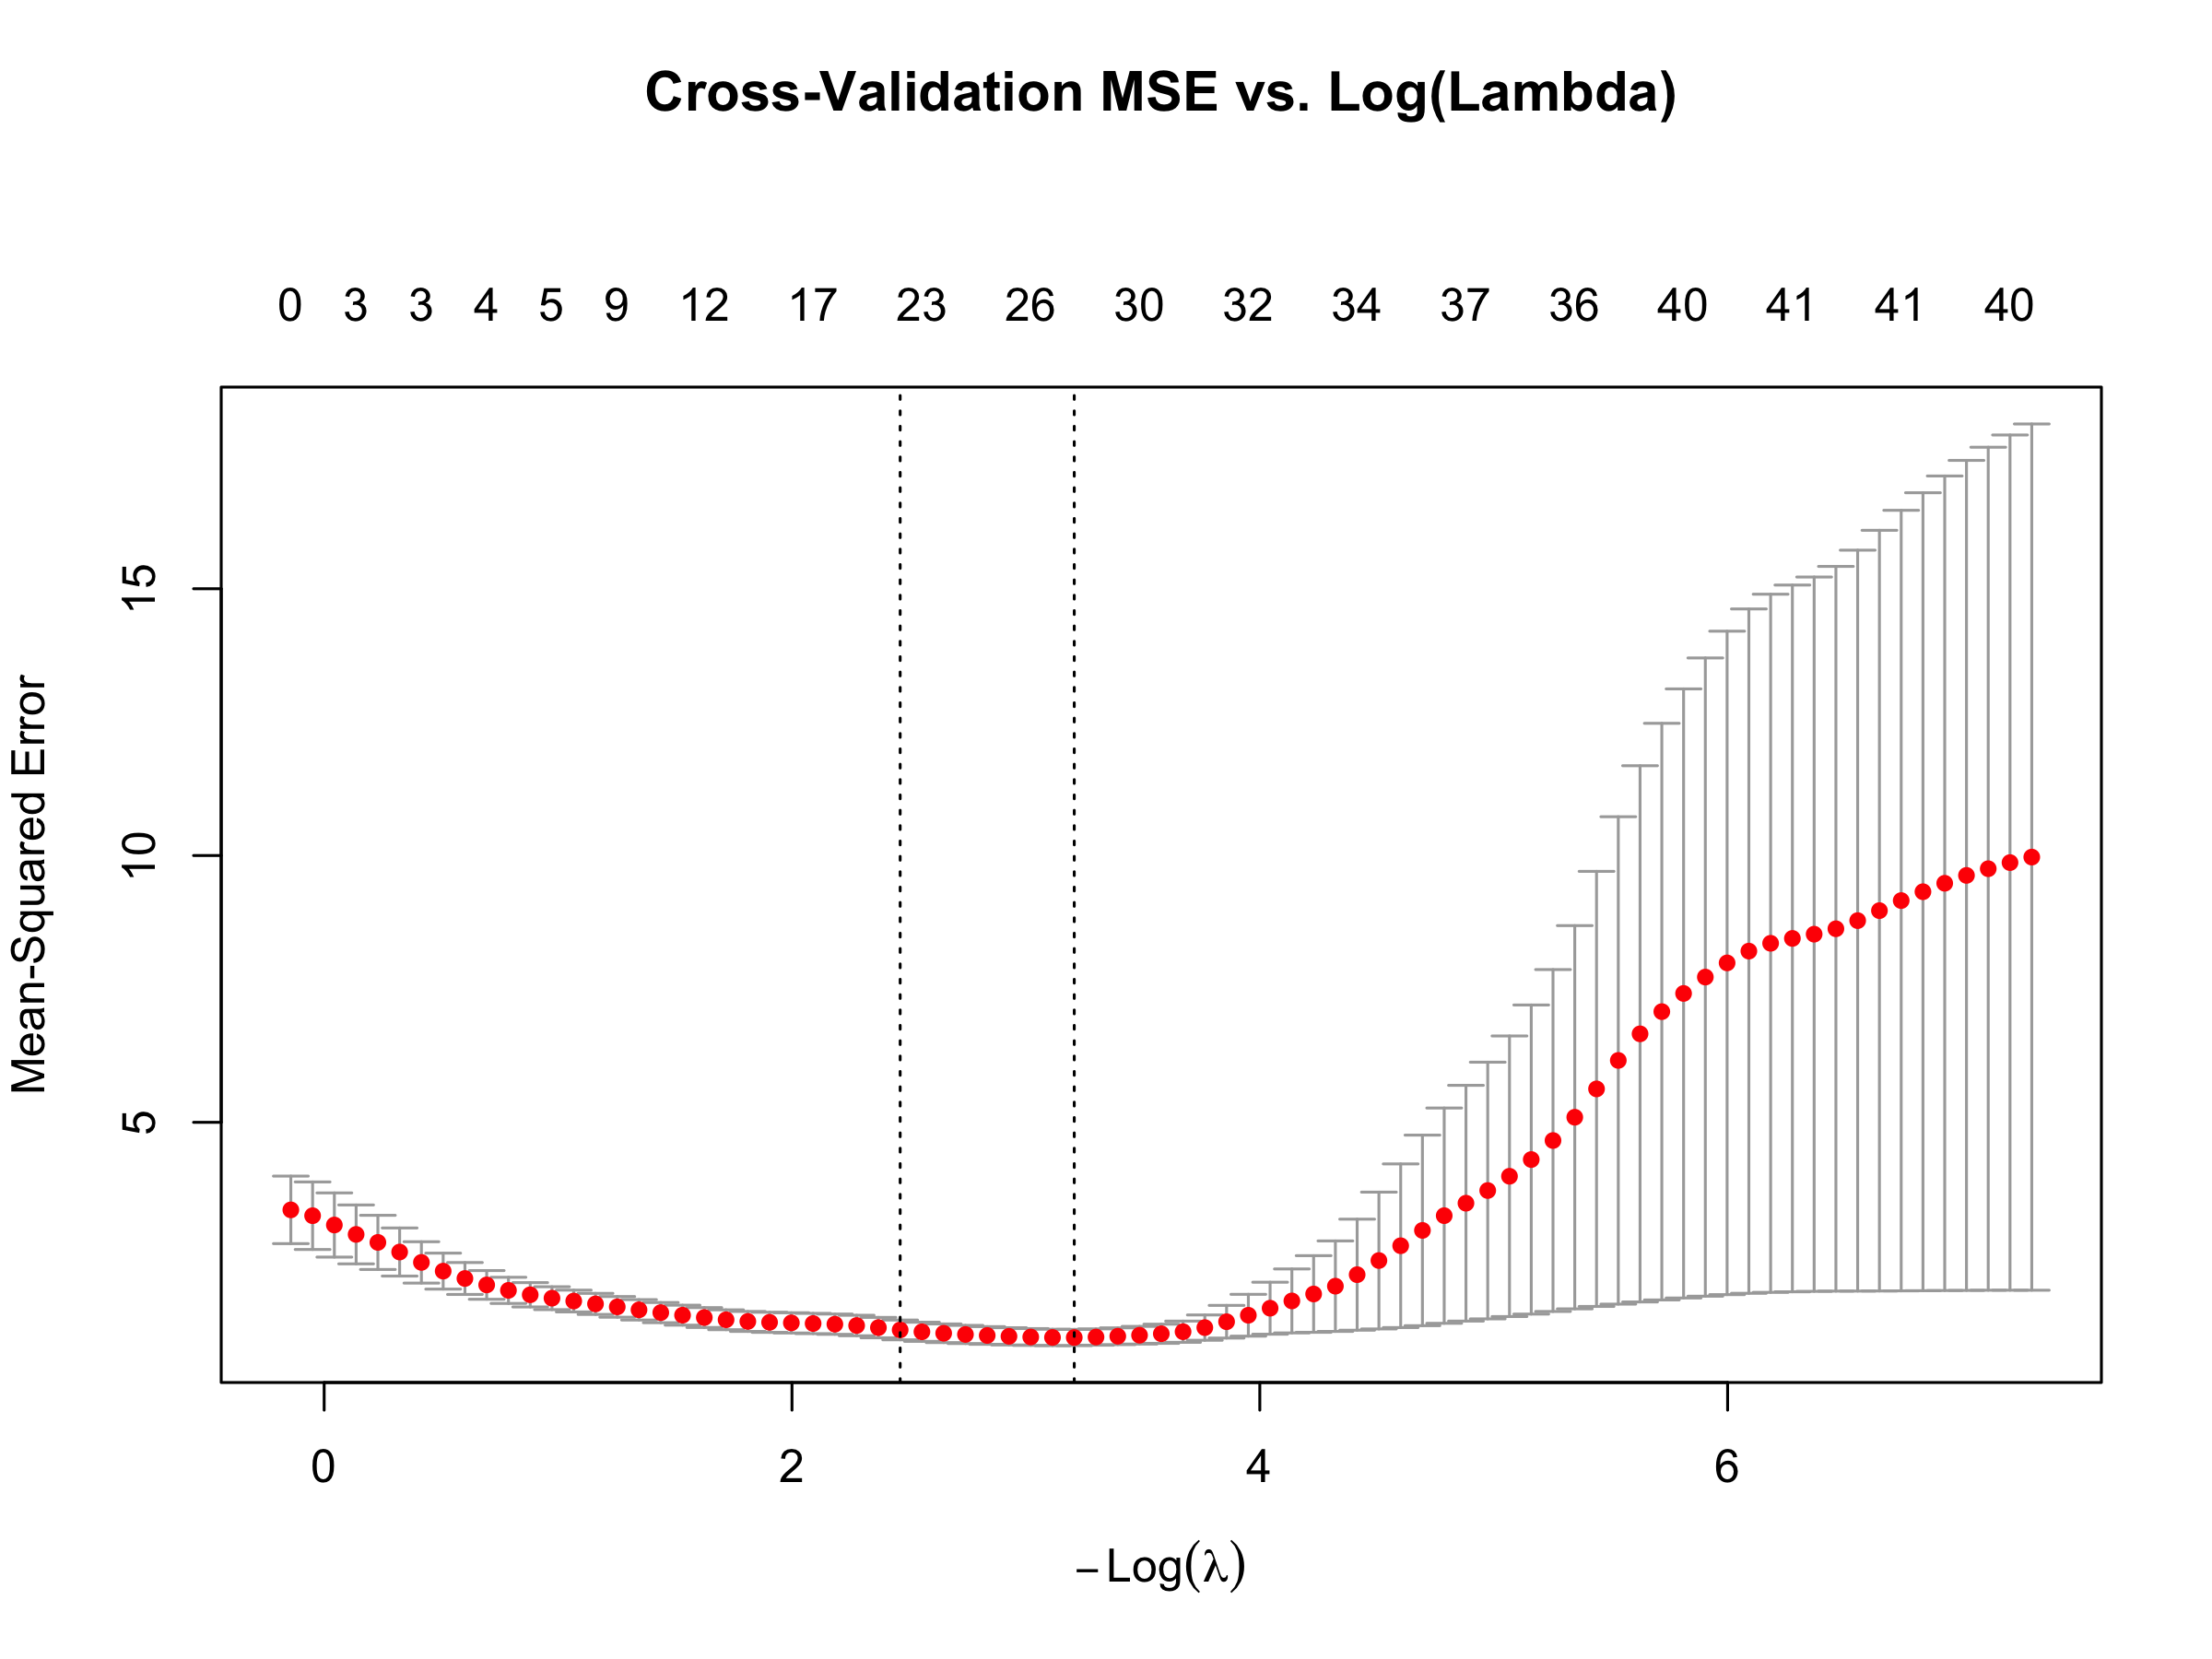
\includegraphics[width=0.85\textwidth]{../output/figures/cv_plot.png}
    \caption{Cross-validation MSE as a function of $-\log(\lambda)$, with the
    number of non-zero coefficients shown along the top axis. The right dotted
    line marks \texttt{lambda.min} ($\lambda = 0.0405$) and the left marks
    \texttt{lambda.1se}. Varian's $\lambda = 0.1489$ falls to the left of both
    lines.}
    \label{fig:cv}
\end{figure}

\subsection*{Updated Model: Top 10 Predictors}

Table~\ref{tab:top10} reports the top 10 predictors ranked by coefficient
magnitude from the updated model. Equipment investment and fraction Confucian
remain the dominant predictors across both versions, with large positive
coefficients. Non-equipment investment (rank 3) and mining (rank 4) also emerge
as important in the updated model, consistent with the broader growth literature
emphasizing physical capital accumulation.

\begin{table}[h]
\centering
\caption{Top 10 Predictors of Economic Growth: Updated LASSO (glmnet 4.1-10)}
\label{tab:top10}
\begin{tabular}{lcc}
\hline
\textit{Rank} & \textit{Predictor} & \textit{Coefficient} \\
\hline
1 & Equip.Inv & $11.9388$ \\
2 & Confuncious & $5.4796$ \\
3 & NEquip.Inv & $4.4918$ \\
4 & Mining & $2.6488$ \\
5 & Buddha & $1.1158$ \\
6 & GDPsh560 & $-1.0406$ \\
7 & Protestants & $-1.0326$ \\
8 & SubSahara & $-0.9987$ \\
9 & Hindu & $-0.6418$ \\
10 & Muslim & $0.629$ \\
\hline
\multicolumn{3}{p{0.75\textwidth}}{\small \textit{Notes:} Coefficients from LASSO with $\lambda = 0.0405$ selected by 10-fold cross-validation using glmnet 4.1-10.}
\end{tabular}
\end{table}


\subsection*{Prediction Error and the Observation 38 Outlier}

Figure~\ref{fig:error} plots the absolute proportional prediction error ---
defined as $|\hat{y}_i - y_i| / |y_i|$, the absolute prediction error
normalized by actual GDP growth --- for each country. The vast majority of
countries have errors below 2, but one observation --- observation 38 --- has
an error of approximately 39, far exceeding all others. At Varian's $\lambda$,
the mean absolute proportional error across all 72 countries is 1.21, but drops
to 0.68 when observation 38 is excluded. Varian himself flags this observation
in his original code but does not identify the country.

Based on the covariate profile of observation 38 --- Latin America dummy = 1,
Spanish colony dummy = 1, war dummy = 1, Catholic fraction = 0.95, and actual
GDP growth of only 0.037\% --- this appears to be a Latin American country that
experienced conflict during 1960--1985 and achieved near-zero growth. LASSO
overpredicted growth for this country by approximately 1.45 percentage points,
which normalized by the near-zero actual growth rate produces the extreme
proportional error of $\approx$39. This suggests the model's selected covariates
could not fully capture the idiosyncratic factors suppressing growth in this case.

\begin{figure}[htbp]
    \centering
    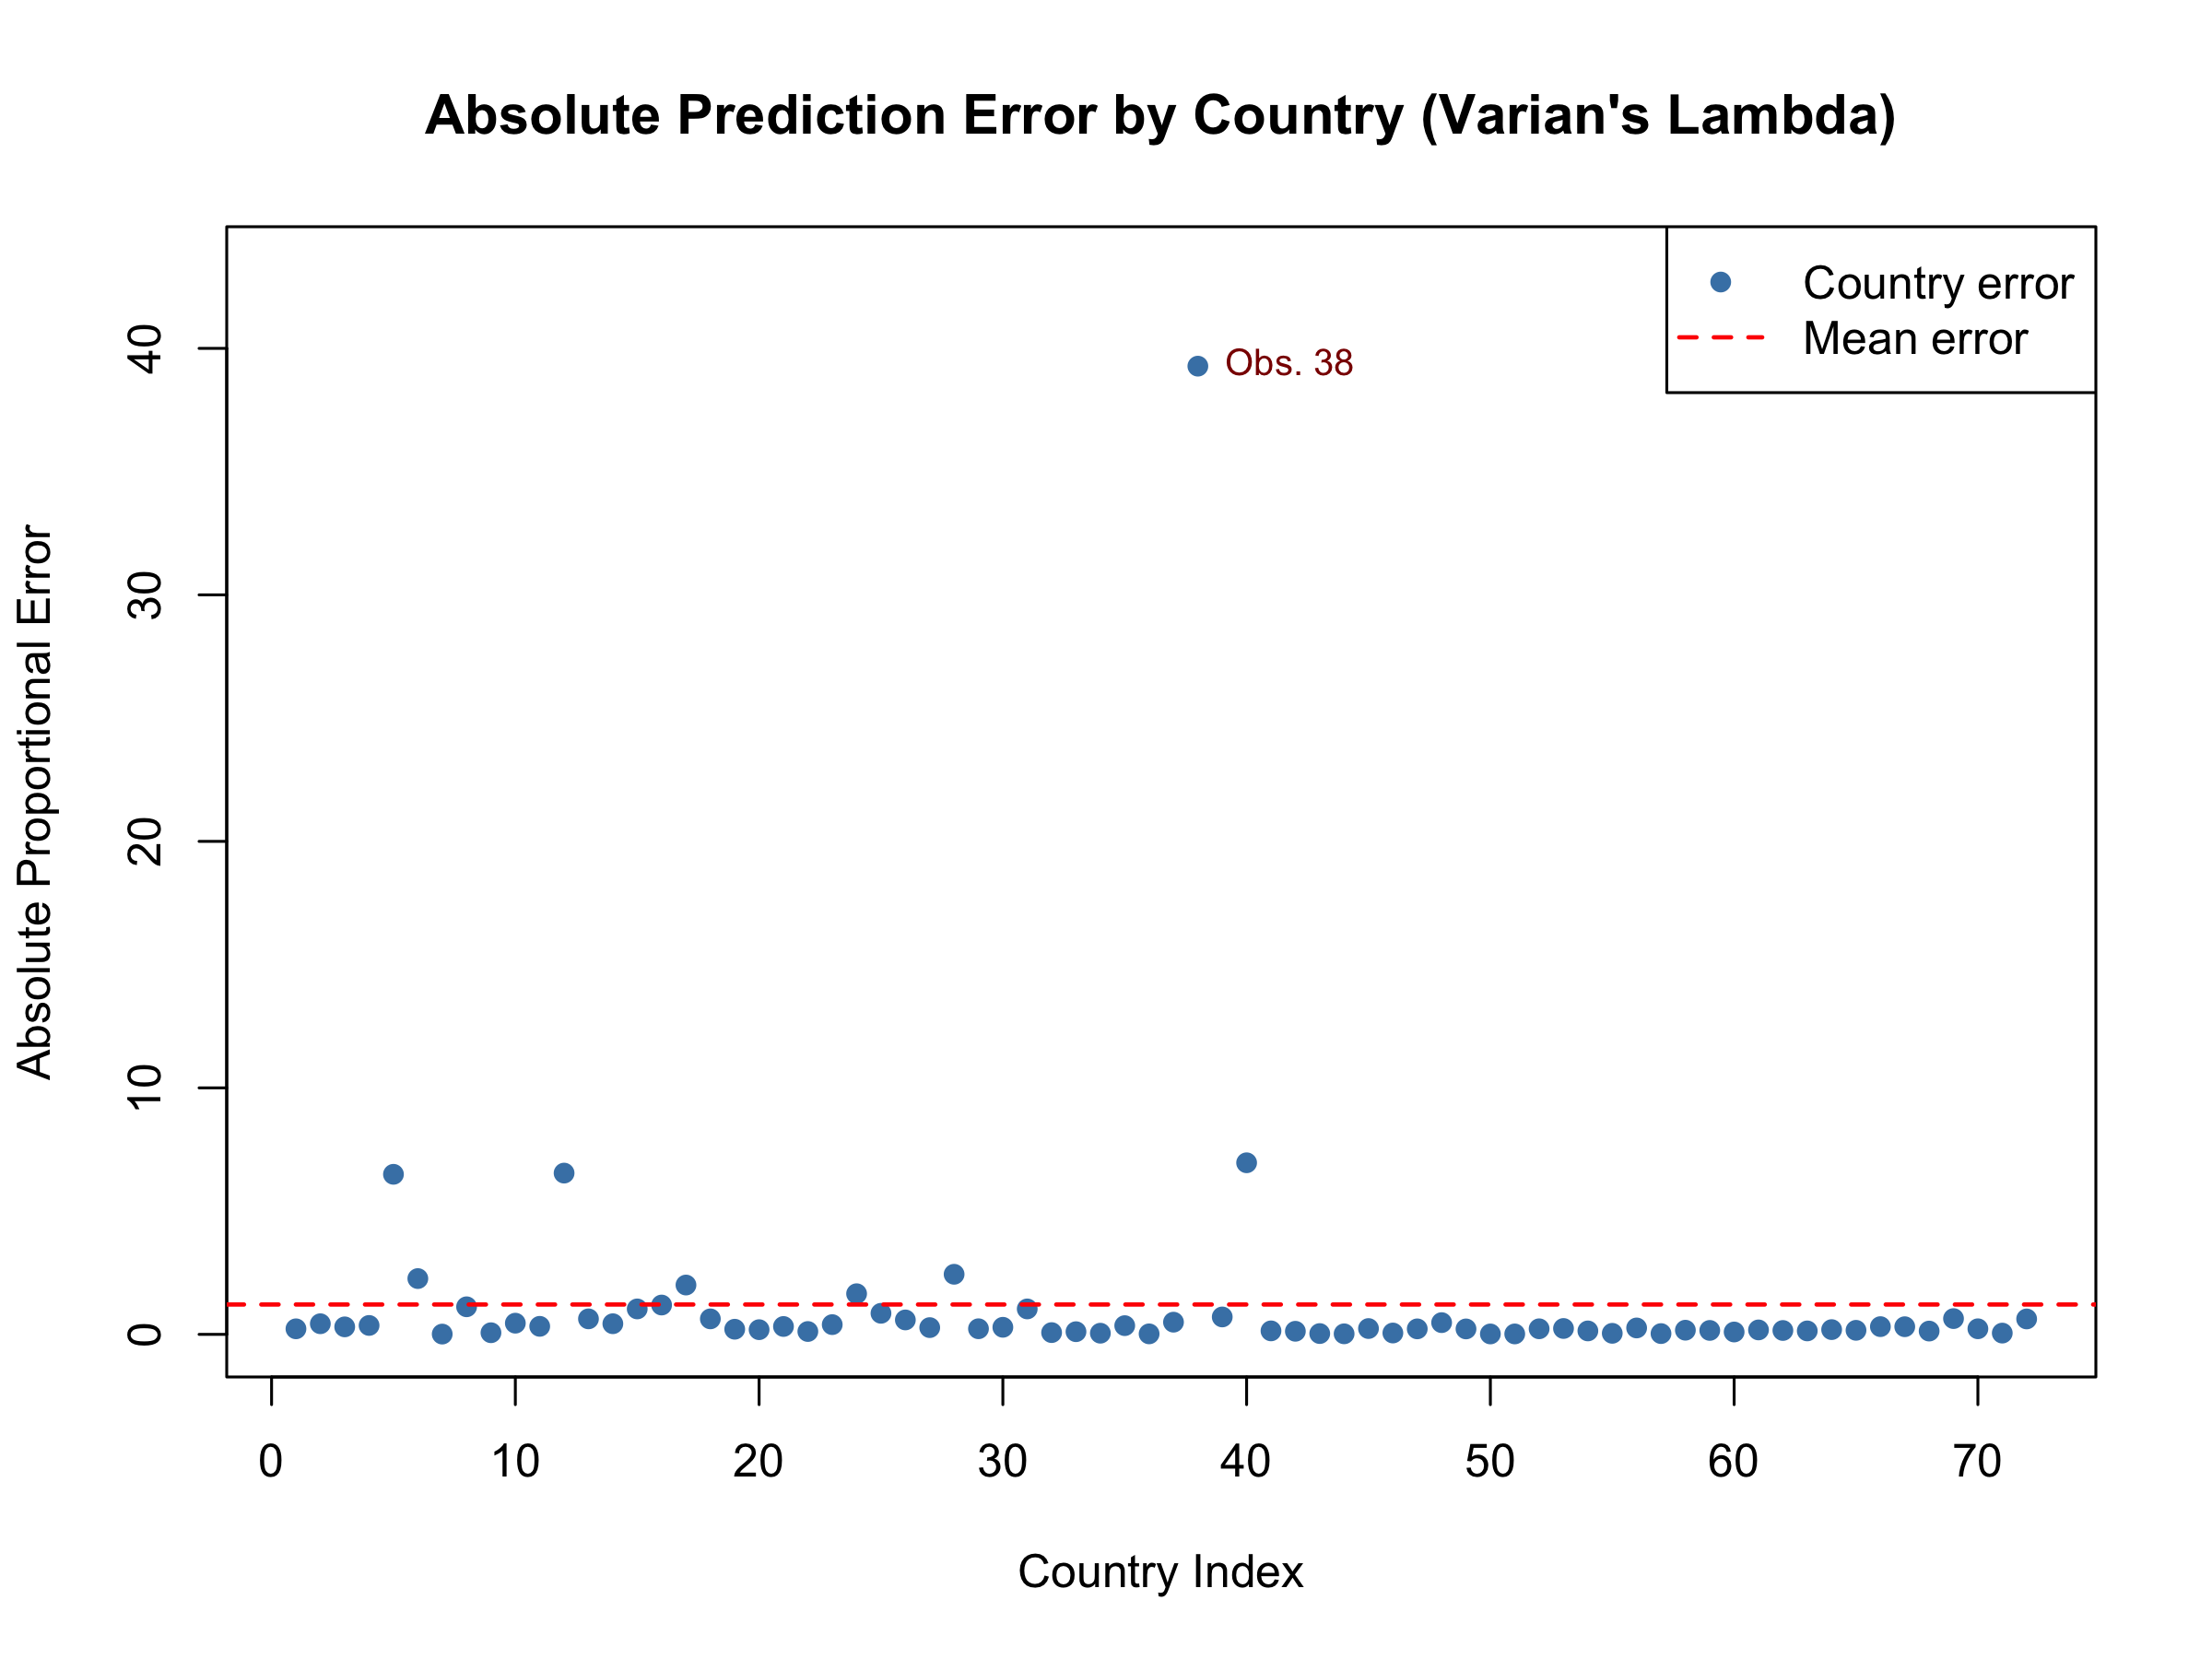
\includegraphics[width=0.85\textwidth]{../output/figures/error_plot.png}
    \caption{Absolute proportional prediction error ($|\hat{y}_i - y_i| /
    |y_i|$) by country at Varian's $\lambda = 0.1489$. Observation 38 is a
    clear outlier, corresponding to a Latin American country with near-zero
    actual GDP growth that LASSO substantially overpredicted. The red dashed
    line shows the mean error across all 72 countries.}
    \label{fig:error}
\end{figure}

% =============================================================================
\section{What I Learned}
% =============================================================================

\textbf{What was easiest.} The data preparation was remarkably straightforward.
The FLS dataset is clean, well-structured, and publicly available --- Varian even
provides his original R scripts, making it easy to verify that our code
faithfully reproduces his steps. The \texttt{glmnet} package abstracts away
most of the numerical complexity, so the core analysis is only a handful of
lines.

\textbf{What was hardest and most interesting.} The most surprising finding was
that running Varian's own code with the current version of \texttt{glmnet}
does not reproduce his results. The cross-validation procedure in
\texttt{cv.glmnet} has changed between the version Varian used (circa 2014) and
the current version (4.1-10), producing a different optimal $\lambda$ (0.0405
vs.\ 0.1489) and a less sparse model (27 vs.\ 14 non-zero coefficients). This
discrepancy arose not from any error in Varian's code or data, but from
legitimate improvements to the package over a decade. This is a vivid
illustration of a well-known problem in computational reproducibility: results
can depend on software versions in ways that are invisible unless you try to
replicate them. If Varian had published a \texttt{sessionInfo()} output or a
Docker container alongside his code, this discrepancy would have been
immediately apparent.

\textbf{What this paper taught me about reproducibility.} Replicating Varian
(2014) clarified for me that reproducibility has two distinct levels: exact
numerical reproducibility (which requires fixing software versions) and
qualitative reproducibility (which is more robust). At the qualitative level,
our replication is a success --- the top predictors of economic growth identified
by LASSO are consistent across both versions, and the core message of the paper
holds. At the exact numerical level, the results differ due to package
evolution. A good replication package should make both levels transparent.

\textbf{Connection to causal machine learning.} Perhaps the most important
thing I learned from this replication is why it matters for causal inference.
Varian (2014) is fundamentally a prediction paper --- LASSO is used to find
which variables best predict economic growth, not to identify causal effects.
But the variable selection step Varian demonstrates is exactly Step 1 of the
Double LASSO estimator (Belloni, Chernozhukov, and Hansen, 2014) and the
Double/Debiased ML framework (Chernozhukov et al., 2018). In those methods,
LASSO is run twice --- once to select controls that predict the outcome, and
once to select controls that predict the treatment --- and the resulting
residuals are used for valid causal inference in high-dimensional settings.
Applied to this dataset, one could use Double LASSO to estimate the causal
effect of equipment investment on economic growth, using the remaining 40
covariates as LASSO-selected controls --- a question Varian's predictive
exercise motivates but does not answer. Varian's paper thus serves as a natural
and accessible motivation for why principled variable selection is a prerequisite
for credible causal inference when $p$ is large relative to $n$.

\textbf{The power of LASSO relative to exhaustive search.} One of the most
striking takeaways from this replication is just how efficient LASSO is as a
variable selection tool. Sala-i-Mart\'{i}n (1997) ran over two million
regressions --- systematically evaluating all manageable subsets of the 41
covariates --- to construct his CDF(0) importance measure. LASSO arrives at
a strikingly similar ranking of important growth predictors by solving a single
penalized regression problem (Equation~\ref{eq:lasso}). The top variables
identified by both approaches overlap substantially, yet LASSO requires a
fraction of the computational resources. This efficiency is not merely
convenient: it scales to settings where exhaustive search is computationally
infeasible, making LASSO practically indispensable for modern high-dimensional
empirical work.

% =============================================================================
\begin{thebibliography}{9}

\bibitem{varian2014}
Varian, Hal R. ``Big Data: New Tricks for Econometrics.''
\textit{Journal of Economic Perspectives} 28, no. 2 (2014): 3--28.

\bibitem{fls2001}
Fernandez, C., Ley, E., and Steel, M. F. J.
``Model Uncertainty in Cross-Country Growth Regressions.''
\textit{Journal of Applied Econometrics} 16, no. 5 (2001): 563--576.

\bibitem{sala1997}
Sala-i-Mart\'{i}n, Xavier.
``I Just Ran Two Million Regressions.''
\textit{American Economic Review} 87, no. 2 (1997): 178--183.

\bibitem{leysteel2009}
Ley, E., and Steel, M. F. J.
``On the Effect of Prior Assumptions in Bayesian Model Averaging with Applications to Growth Regression.''
\textit{Journal of Applied Econometrics} 24, no. 4 (2009): 651--674.

\bibitem{belloni2014}
Belloni, A., Chernozhukov, V., and Hansen, C.
``High-Dimensional Methods and Inference on Structural and Treatment Effects.''
\textit{Journal of Economic Perspectives} 28, no. 2 (2014): 29--50.

\bibitem{chernozhukov2018}
Chernozhukov, V., Chetverikov, D., Demirer, M., Duflo, E., Hansen, C.,
Newey, W., and Robins, J.
``Double/Debiased Machine Learning for Treatment and Structural Parameters.''
\textit{The Econometrics Journal} 21, no. 1 (2018): C1--C68.

\end{thebibliography}

\end{document}
